\documentclass[a0,portrait]{a0poster}
\usepackage[dvips,usenames]{color}
\usepackage{a0size}
\usepackage{times}
\usepackage{graphicx}
\usepackage[latin2]{inputenc}
\usepackage{xcolor}
\usepackage{pgfplots}
\usepackage{tikzscale}
\usepackage{listings}

\usepackage[T1]{fontenc}
\usepackage{mathtools}
\usepackage{amsfonts}
\usepackage{amsmath}
\usepackage{tabu}
\usepackage{caption}
\usepackage{multirow}
\usepackage{booktabs}
\usepackage{amssymb,amsthm}
\usepackage{graphicx}
\usepackage{diagbox}
\usepackage{float}

\usepackage{breakurl}   
\usepackage{hyperref}
%%\usepackage[T1]{fontenc}
%%\usepackage[ttdefault=true]{AnonymousPro}
\usepackage{inconsolata}
\usepackage[T1]{fontenc}


\usepackage{listings}
%\usepackage{color}

\lstdefinelanguage{Clean}{%
    alsoletter={ABCDEFGHIJKLMNOPQRSTUVWXYZabcdefghijklmnopqrstuvwxyz_^`},%
    alsoletter={~!@\#\$\%^\&*-+=?<>:|\\.},%
   morekeywords={generic,implementation,definition,dynamic,module,import,from,while,then,else,where,in,of,case,let,infix,infixr,infixl,class,instance,with,if,derive,otherwise},%
%    otherkeywords={=,.,!,|,\&,\#,\\,=>,->,::,=:,\\\\,:==},%
    sensitive=true,%
    morecomment=[l]{//},%
    morecomment=[n]{/*}{*/},%
    morestring=[b]",%
    morestring=[b]',%
    emptylines=1,%
%    basicstyle=\scriptsize,%
    basicstyle=\small,%
%    identifierstyle=\sffamily,%
    identifierstyle=\ttfamily,%
    commentstyle=\itshape,%
    keywordstyle={\sffamily\bfseries},%
%    keywordstyle={\ttfamily\bfseries},%
    stringstyle=\ttfamily,%
    numbers=none,%
    showstringspaces=false,%
%    basewidth=0.50em,%
    basewidth=0.50em,%
    columns=[c]fixed,%
    keepspaces=true,%
    breaklines=false,%
%    breakindent=40pt,%
%    prebreak={\space...},%
%    postbreak={...\space},%
    tabsize=2,%
    texcl=true,%
    escapeinside={(\#}{\#)},%
    literate=   {\\}{{$\lambda$}}1%
                {A.}{{$\forall$}}1%
                {E.}{{$\exists$}}1%
                {<=}{{$\leq$}}1%
                {>=}{{$\geq$}}1%
                {<>}{{$\neq$}}1%
                {->}{{$\rightarrow$}}2%
                {|->}{{$\mapsto$}}2%
                {=}{{$=$}}1%
                {=>}{{$\Rightarrow$}}2%
                {<-}{{$\leftarrow$}}2%
                {==}{{${=\!\!\!=}$}}2%
                {=->}{{$\Rrightarrow$}}2%
                {==>}{{$\Longrightarrow$}}3%
%                {~}{{$\neg$}}1%
                {~~}{{$\approx$}}2%
                {~/~}{{$\ncong$}}2%
                {<~}{{$\lesssim$}}2%
                {</~}{{$\lesssim\!\!\!\!\!/\ $}}2%
                {\#}{{$\sharp$}}1%
                {\{|}{{$\!\{\!|$}}1%
                {|\}}{{$\,|\!\}$}}1%
                {<->}{{$\leftrightarrow$}}2%
                {<|>}{{$\updownarrow$}}2%
                {/.\\}{{$\wedge\!\!\!.\,$}}1%
                {/\\}{{$\wedge$}}1%
                {\\./}{{$\vee\!\!\!\cdot\,$}}1%
                {\\.n}{$\backslash$n}2%
                {\\n}{$\backslash$n}2%
                {\\"}{$\backslash$"}2%
                {\\t}{$\backslash$t}2%
                {\\\\t}{$\backslash$t}2%
                {\\\\}{$\backslash$t}1%
                {>>>}{{$>\!\!>\!\!>$}}2%
                {>>==}{{$>\!\!>==$}}5%
                {>>=}{{$>\!\!>=$}}3%
                {>>=.}{{$>\!\!>=\mathbf{.}$}}4%
%                {>>=.}{{$>\!\!>=\mathbf{.}$}}5%
                {:.}{{$:\!.$}}2%
                {***}{{$*\!\!*\!\!*$}}2%
                {\&\&\&}{{$\&\!\!\&\!\!\&$}}2%
                {<<<}{{$<\!\!<\!\!<$}}2%
                {\{|*|\}}{{$\{\!|\!\!\star\!\!|\!\}$}}3%
}%
%
\lstdefinestyle{numbers}{numbers=right, stepnumber=1, numberstyle=\tiny, numbersep=-7pt}
\lstnewenvironment{CleanCode}{\lstset{language=Clean}}{}%
\lstnewenvironment{CleanCodeN}{\lstset{language=Clean,style=numbers}}{}%
\lstnewenvironment{CleanCodeNB}{\lstset{language=Clean,style=numbers,frame=single}}{}%
\lstnewenvironment{CleanCodeB}{\lstset{language=Clean,frame=single}}{}%
%
\newcommand{\CleanInline}[1]{\lstinline[language=Clean]$#1$}%
\newcommand{\Cl}[1]{\lstinline[language=Clean]$#1$}%
\newcommand{\prog}[1]{\lstinline[language=Clean]$#1$}%


\lstset{language=C++,
        basicstyle=\footnotesize\ttfamily,
        keywordstyle=\color{blue}\ttfamily,
        stringstyle=\color{red}\ttfamily,
        commentstyle=\color{green!40!black}\ttfamily,
        morecomment=[l][\color{magenta}]{\#}
}

%\pgfplotsset{compat=1.15}

\usepgfplotslibrary{units}
\usetikzlibrary{arrows, positioning}
\usetikzlibrary{shapes}

\setcounter{secnumdepth}{0}
\pagestyle{empty}
\renewcommand{\thefootnote}{\fnsymbol{footnote}}
\definecolor{title}{named}{BrickRed}
\definecolor{sect}{rgb}{0,0,0.7}
\definecolor{proof}{rgb}{0.7,0,0}

\definecolor{custom}{HTML}{3388aa}
\definecolor{coffee}{HTML}{C0FFEE}
\definecolor{blackk}{HTML}{000000}
\definecolor{mycolor}{HTML}{3388aa}

\usepackage{filecontents}

\begin{document}

\newcommand{\sect}[1]{\vspace{3cm}
  {\color{sect}\LARGE\itshape\bfseries #1}\vspace{2cm}}
\newcommand{\ssect}[1]{{\color{custom}\Large\bfseries #1}\vspace{0.6 cm}

}
\newenvironment{sectbox}{
\begin{minipage}[t]{0.45\textwidth}
\addtolength{\parskip}{0.5\baselineskip}
}{
\end{minipage}
}
\vspace{1.0cm}
\begin{center}
{\Huge\bfseries\sffamily\color{custom} {Implementation of Digital Synthesis in Functional Programming}}\\
\vspace{1.5cm}
{\LARGE\color{blackk} Xiaotian Su, Evan Sitt, Beka Grdzelishvili, Zurab Tsinadze, Zongpu Xie}\\{\LARGE\color{blackk} Hossameldin Abdin, Giorgi Botkoveli, Nikola Cenikj, Tringa Sylaj, Vikt\'oria Zs\'ok}\\
\vspace{1.2cm}
{\large\color{blackk} {\{suxiaotian31, sitt.evan, bekagrdzelishvili0, zukatsinadze, szumixie, hossamabdeen17, botko.gio, nicola.cenic,  tringasylaj\}@gmail.com, zsv@inf.elte.hu}}\\
\vspace{1.2cm} %\textsuperscript{1}
{\large  \color{blackk}
E\"otv\"os Lor\'and University, Faculty of Informatics\\
Department of Programming Languages and Compilers\\
H-1117 Budapest, P\'azm\'any P\'eter s\'et\'any 1/C., Hungary}\\
%\vspace{0.3cm}
%{\Large \textsuperscript{2} Ericsson Ltd.\\
%        Magyar tud\'osok k\"or\'utja, 11., Budapest, Hungary}
\end{center}
\hspace{0.01\textwidth}
\begin{sectbox}
\ssect{Introduction}

\emph{Digital Synthesis} is a \emph{digital signal processing}
technique for creating musical sounds. In contrast to analog synthesizers, digital synthesis processes discrete bit data to replicate and recreate a continuous waveform.
The digital signal processing techniques used are relevant in many disciplines and fields including telecommunications, biomedical engineering, and seismology.

\vspace{1cm}

\ssect{Motivation}
We chose to pursue this project in order to extend the possible applications that can be created with the pure lazy functional programming \emph{Clean} language \cite{clean}. The language offers very good abstractions tools for sound generation implementation. Digital synthesis is typically accomplished within a \emph{C++} framework, however the nature of synthesis involving multiple tracks and post-processes in parallel lends itself naturally to a functional programming paradigm \cite{organ}.

\vspace{1cm}

\ssect{Wavetable Lookup Synthesis}
In implementing the digital synthesis, we utilized a technique called \emph{Wavetable Lookup Synthesis}, in which a certain waveform is stored in a wavetable with constant access, and exploit the relation between frequency and sampling rate to quickly build new waveforms. We used a single cycle (shown in Figure \ref{fig:sineWavetable}) sine wavetable as the basis for our additive and subtractive synthesis, utilizing Fourier series of sine functions to generate all other waveforms.

\begin{figure}[H]
  \centering
  \begin{minipage}[b]{0.5\textwidth}
    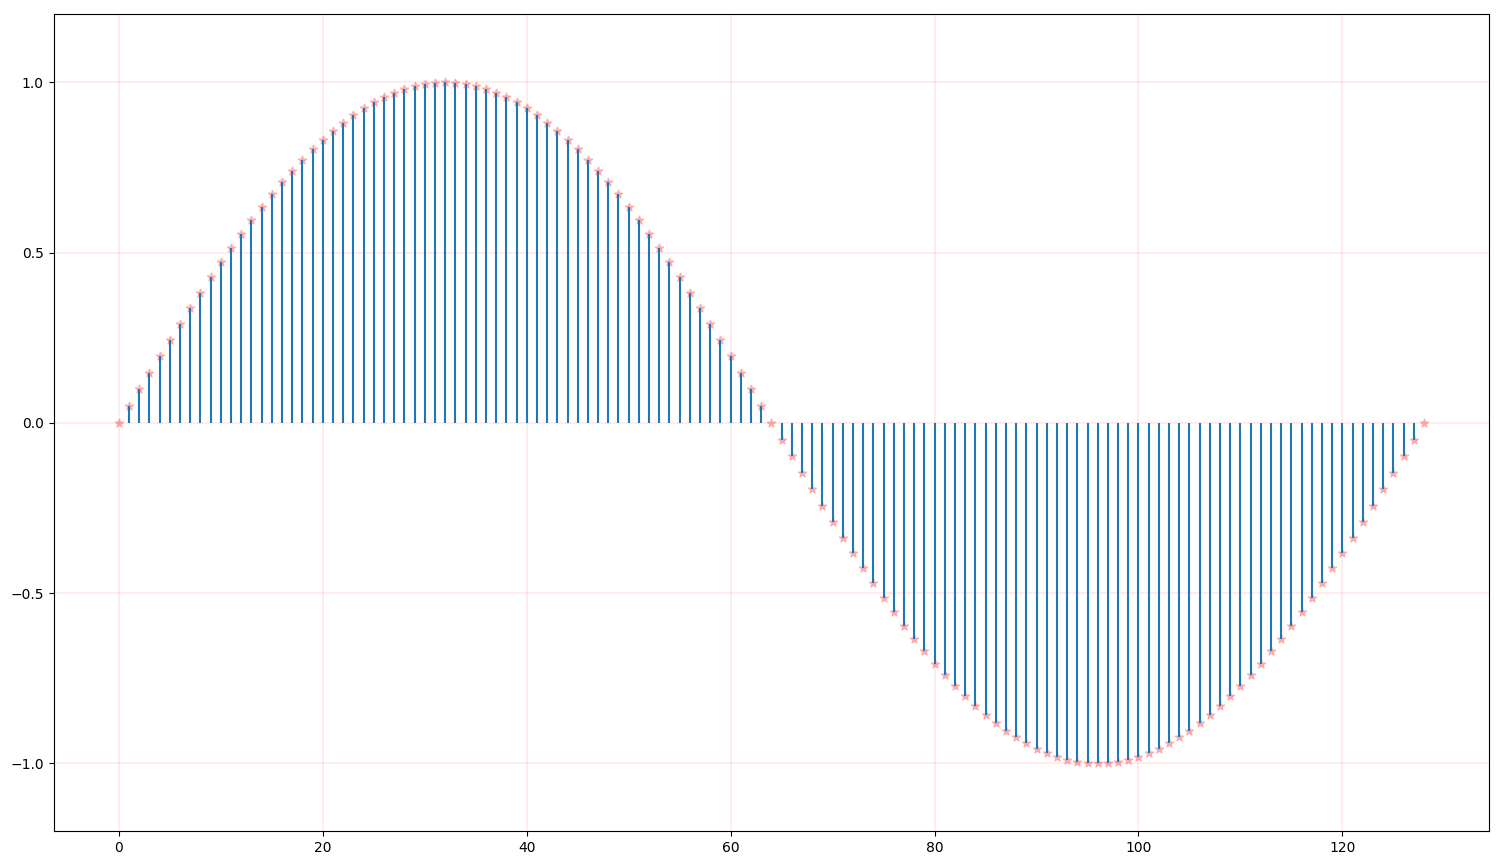
\includegraphics[width=\textwidth]{wavetable.png}
    \caption{Single Cycle Sine Wavetable}
    \label{fig:sineWavetable}
  \end{minipage}
  \hfill
\end{figure}
From the simple sine wave, we then do a weighted summation of harmonics to generate more sophisiticated waveforms. An example can be seen in Figure \ref{fig:sawtoothWaveform} where a sawtooth was generated. The sawtooth waveform was then further used with subtractive synthesis to generate the pulse waveform shown in Figure \ref{fig:pulseWaveform}.
\begin{figure}[H]
  \centering
  \begin{minipage}[b]{0.45\textwidth}
    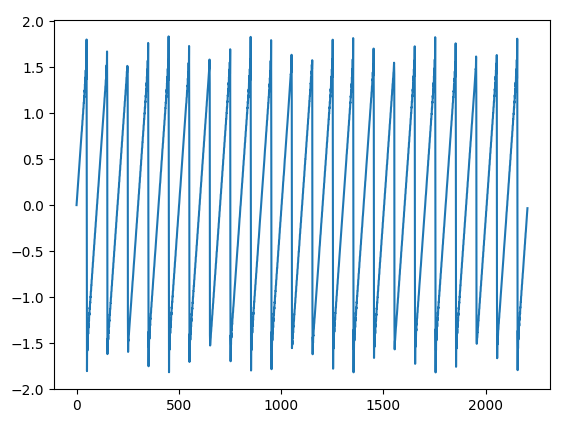
\includegraphics[width=\textwidth]{saw.png}
    \caption{Sawtooth Waveform}
    \label{fig:sawtoothWaveform}
  \end{minipage}
  \hfill
  \begin{minipage}[b]{0.45\textwidth}
    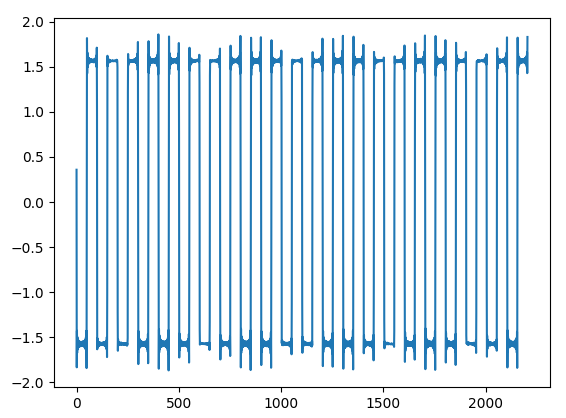
\includegraphics[width=\textwidth]{pulse.png}
    \caption{Pulse Waveform}
    \label{fig:pulseWaveform}
  \end{minipage}
\end{figure}

\vspace{1cm}

\ssect{Envelope}

After generating the waveforms, we can further post-process the data with effects and filters. The effect we chose to implement was the envelope, starting first with the standard 4-step ADSR envelope, and then later proceeding to a more sophisticated 6-step DAHDSR envelope.\\
The basic 4-step ADSR envelope is shown below in Figure \ref{fig:ADSR}, illustrating the multiplier values. A more sophisticated 6-step DAHDSR envelope applied to a standard sine waveform is shown in Figure \ref{fig:DAHDSR}.\\

\begin{figure}[H]
  \centering
  \begin{minipage}[b]{0.45\textwidth}
    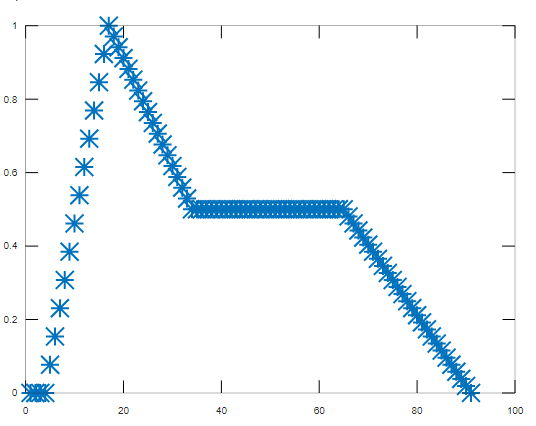
\includegraphics[width=\textwidth]{ADSR.png}
    \caption{4-Step ADSR Envelope}
    \label{fig:ADSR}
  \end{minipage}
  \hfill
  \begin{minipage}[b]{0.45\textwidth}
    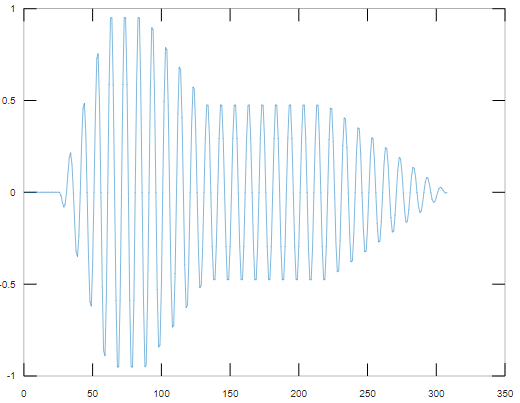
\includegraphics[width=\textwidth]{DAHDSR.png}
    \caption{6-Step DAHDSR Envelope}
    \label{fig:DAHDSR}
  \end{minipage}
\end{figure}
This code illustrates how list comprehensions are used extensively to render the MIDI event messages into processed waveforms.
\begin{CleanCode}
render :: [NoteChunk] -> [Real]
render chunkList = normalized
where
	totalSamples = maxList [numberOfSamples x (x.note.initialTime+x.note.duration) \\x <- chunkList]
	silenceTrack = generateSilence totalSamples
	renderedTrack = [(generateSilence (numberOfSamples x x.note.initialTime))++(renderNoteChunk x)++                 
	                 (generateSilence (totalSamples - (numberOfSamples x (x.note.initialTime +
	                 x.note.duration)))) \\ x <- chunkList]
	renderedTrackArr = [listToArr ls \\ ls <- renderedTrack]
	noteSum = [(sum [arr.[ind] \\ arr <- renderedTrackArr]) \\ ind <- [0,1..(totalSamples-1)]]
	normalized = normalizeList noteSum
\end{CleanCode}

\end{sectbox}
% -----------------------------------------------------------------------------
\hspace{0.03\textwidth}
%
\begin{sectbox}

\ssect{MIDI Input}
MIDI is short for Musical Instrument Digital Interface which related audio devices for playing, editing and recording music.MIDI carries event messages, data that specify the instructions for music, including note on, note off events, velocity,etc.

\vspace{1em}
\begin{table}[H]
    \centering
    \taburulecolor{mycolor}
	\begin{tabu}{|l|m{7em}|m{4em}|m{4em}|m{4em}|}
	    \hline
	    \diagbox[width=7.8em,linecolor=mycolor]{\bfseries event type}{\bfseries structure} 
	    & status byte & byte2 & byte3 & byte4 \\
        \hline
		midi events & 0x8n - 0xEn & data & (data) & $-$\\ 
		\hline
		sysex events & 0xF0 and 0xF7 & length & data & $-$\\  
		\hline
		meta events & 0xFF & type & length & data \\  
		\hline
	\end{tabu}
	\captionof{table}{Three types of MIDI Events}
\end{table}

The general structure of the MIDI import functions.
\begin{figure}[H]
  \centering
    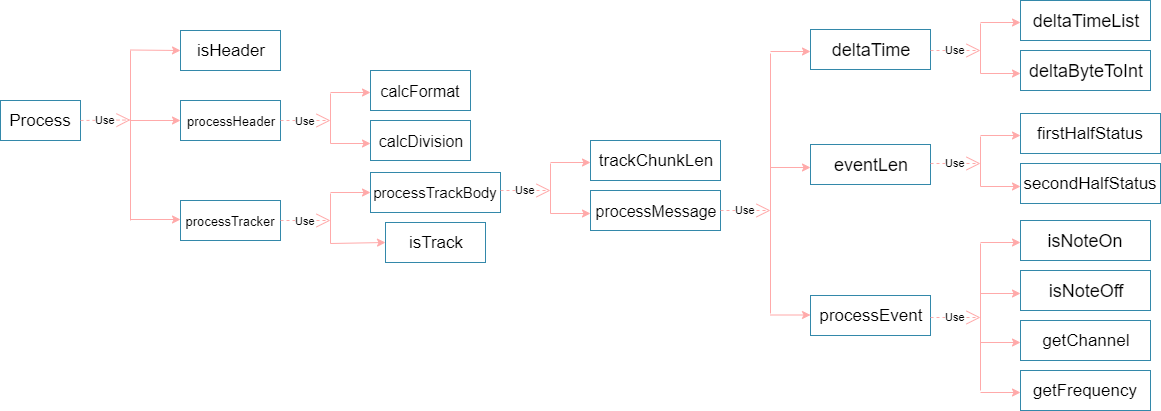
\includegraphics[width=1.0\textwidth]{functions.png}
    \caption{Relations of the functions}
\end{figure}

This code calculates the cumulative time from the beginning of track to the current event. It utilizes the power of pattern matching in functional programming to handle event messages.\\
\begin{figure}[H]
    \centering
    \begin{minipage}{0.5\textwidth}
        \begin{CleanCode}
        findDeltaTime :: Real TrackInfo -> Int
        findDeltaTime _ [] = 0
        findDeltaTime f l
            #! {deltaTime,event} = hd l  
            #! fre = case event of
            	NoteOff a b c -> b
            	_ -> -1.0
            |f == fre = deltaTime
            = deltaTime + findDeltaTime f (tl l)
        \end{CleanCode}
    \end{minipage}
\end{figure}


\ssect{WAV Output}
The Waveform Audio File Format (WAV) follows the RIFF specification, thus the file consists of a header followed by ``subchunks''. A typical WAV file has two subchunks, the first one contains file metadata, the second one consists of the sound data in samples, where each sample is split into channels.

\begin{table}[H]
  \centering
  \taburulecolor{mycolor}
  \newcolumntype{C}{>{\centering\arraybackslash}p{2em}}

\begin{tabu}{|*{12}{C}|}
% \begin{tabu} to 20cm {|*{12}{X[c]}|}
\hline
\multicolumn{12}{|c|}{chunk descriptor} \\ \hline
52 & 49 & 46 & \multicolumn{1}{C|}{46} & 24 & 08 & 00 & \multicolumn{1}{C|}{00} & 57 & 41 & 56 & 45 \\
R & I & F & \multicolumn{1}{C|}{F} & \multicolumn{4}{c|}{chunk size} & W & A & V & E \\ \hline
\multicolumn{12}{|c|}{fmt subchunk} \\ \hline
66 & 6d & 74 & \multicolumn{1}{C|}{20} & 10 & 00 & 00 & \multicolumn{1}{C|}{00} & 01 & \multicolumn{1}{C|}{00} & 02 & 00 \\
f & m & t & \multicolumn{1}{C|}{ } & \multicolumn{4}{c|}{subchunk size} & \multicolumn{2}{c|}{format} & \multicolumn{2}{c|}{channels} \\ \hline
\multicolumn{12}{|c|}{fmt subchunk} \\ \hline
22 & 56 & 00 & \multicolumn{1}{C|}{00} & 88 & 58 & 01 & \multicolumn{1}{C|}{00} & 04 & \multicolumn{1}{C|}{00} & 10 & 00 \\
\multicolumn{4}{|c|}{sample rate} & \multicolumn{4}{c|}{byte rate} & \multicolumn{2}{c|}{block} & \multicolumn{2}{c|}{bits} \\ \hline
\multicolumn{12}{|c|}{data subchunk} \\ \hline
64 & 61 & 74 & \multicolumn{1}{C|}{61} & 00 & 08 & 00 & \multicolumn{1}{C|}{00} & 00 & \multicolumn{1}{C|}{00} & 00 & 00 \\
d & a & t & \multicolumn{1}{C|}{a} & \multicolumn{4}{c|}{subchunk size} & \multicolumn{4}{c|}{sample 1} \\ \hline
\multicolumn{12}{|c|}{data subchunk} \\ \hline
24 & \multicolumn{1}{C|}{17} & 1e & \multicolumn{1}{C|}{f3} & 3c & \multicolumn{1}{C|}{13} & 3c & \multicolumn{1}{C|}{14} & \multicolumn{4}{c|}{$\ldots$} \\
\multicolumn{4}{|c|}{sample 2} & \multicolumn{4}{c|}{sample 3} & & & & \\ \hline
\end{tabu}

  \captionof{table}{Wave File Specification}
\end{table}

% \begin{CleanCode}
% writeFormat :: !PcmWavParams !*File -> *File
% writeFormat p f
%   #! f = fwrites "fmt " f
%   #! f = writeUint 4 16 f // Size of the format block
%   #! f = writeUint 2 1 f // Audio format: PCM
%   #! f = writeUint 2 p.numChannels f
%   #! f = writeUint 4 p.samplingRate f
%   #! f = writeUint 4 (p.samplingRate * p.bytesPerSample * p.numChannels) f
%     // Bytes per second
%   #! f = writeUint 2 (p.bytesPerSample * p.numChannels) f // Bytes per block
%   #! f = writeUint 2 (8 * p.bytesPerSample) f // Bits per sample
%   = f
% \end{CleanCode}


% \vspace{1cm}
\ssect{Conclusion}
The project so far has been successful in meeting the milestones established. We have successfully generated all of the basic waveforms including sine, square, triangle, pulse, sawtooth, and noise. Additionally, we have been able to successfully read event messages from a MIDI file and render out a rendition of the song into a .wav file. 

\vspace{1cm}

\ssect{Acknowledgement} This work was supported by the European Union, co-financed by the European Social Fund, grant. no \textbf{EFOP-3.6.3-VEKOP-16-2017-00002.}

\nocite{*}
%\bibliographystyle{eptcs}
\color{custom}
\begin{thebibliography}{199}\label{bibi}
\color{blackk}
\bibitem{clean} Clean Language Report, \url{https://clean.cs.ru.nl/download/doc/CleanLangRep.2.2.pdf}.

\bibitem{music} Hudak, P., Quick, D.: Haskell School of Music -- From Signals to Symphonies,
\emph{Cambridge University Press}, 2018.

\bibitem{thompsons} Thompson, S.: The Haskell: The Craft of Functional Programming, 
\emph{ Addison-Wesley Professional}, 3rd edition, 2011.

\bibitem{organ} Zuurbier, E.: Organ Music in Just Intonation, \url{https://www.ji5.nl/}.
\end{thebibliography}


%ANNOTATION STUFF GOES HERE
% This work was supported by the European Union,
% co- financed by the European Social Fund,
% grant. no EFOP-3.6.3-VEKOP-16-2017-00002.

\end{sectbox}

\end{document}